\section{Convergence Properties}

To demonstrate the convergence properties of both the original and subsampled schemes, we use a two dimensional set-up similar to Fig. \ref{fig:gradient}, but aligned diagonally across the pixel grid to further expose issues when assigning the contribution of a whole particle to a single pixel. Here the inter-particle spacing runs from $10^{-3}$ to $10^{-2.5}$ linearly across the space, but now the field is extended so that it covers the second dimension in the plane. The particle positions are then rotated $45^\circ$ so that their spacing is not aligned with the pixel grid.

\begin{figure*}
  \centering
  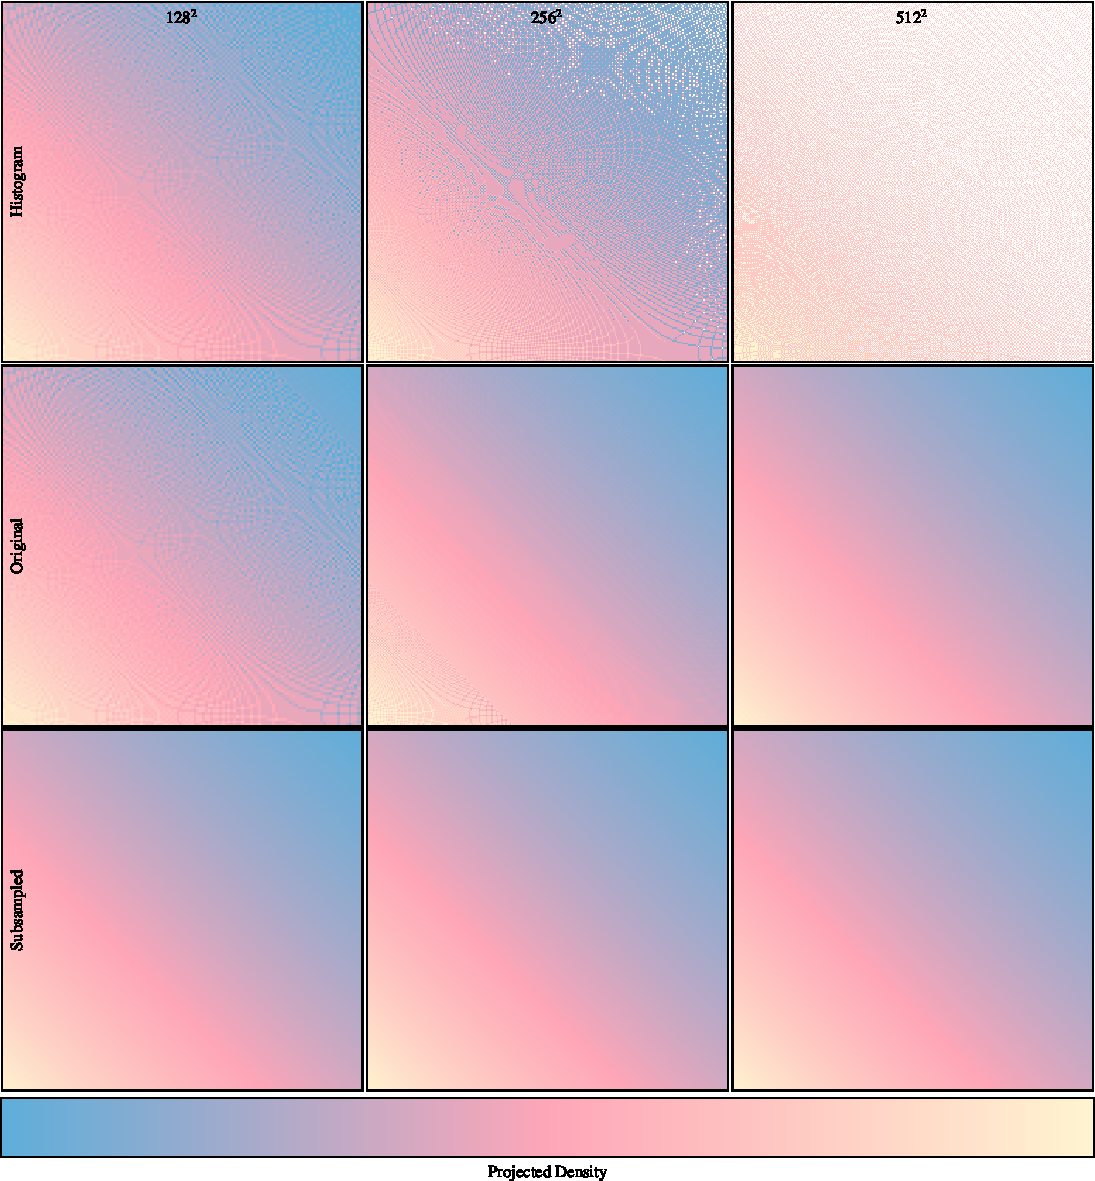
\includegraphics[width=\textwidth]{./plots/gradient_2d/gradients_2d.pdf}
    \caption{A linear (diagonal) gradient in smoothing length from $10^{-3}$ to $10^{-2.5}$ (in units of the box-size) projected with three different methods (rows) at three different grid resolutions (columns). Here the top method is a simple histogram, where each particle is assigned to its nearest grid centre; this is to demonstrate the basic Moir\'e pattern generated when the grid resolution is close to the particle spacing. The centre row shows how this pattern is also present when using the original scheme for particles below the resolution limit, with the bottom row showing the same gradient for each resolution and demonstrating that the subsampled technique can remove all such patterns. These visualisations are used in Fig. \ref{fig:gradconv} to demonstrate the convergence and costs (Fig. \ref{fig:gradtime}) of each method.}
  \label{fig:gradient2d}
\end{figure*}

The projected densities from this plane are shown in Fig. \ref{fig:gradient2d} using three methods, and three resolutions. The first method, on the top row, only ever uses direct particle assignment to the pixels, and as such is simply a two dimensional histogram. This is provided for comparison with the next two rows that employ the original smoothing scheme and the subsampled scheme. The histogram demonstrates the Moir\'e patterns that occur when the particle distribution and the grid spacing do not align, which would lead to large reconstruction errors.

Those same Moir\'e patterns are shown in the centre-left panel where the original scheme is used with the particle distribution to calculate projected densities on a $128^2$ pixel grid. The subsampled approach, however, does not show any such patterns, mainly due to the use of the blitting grid.

The centre column, calculated on a $256^2$ grid, enables the majority of the particles to have smoothing lengths large enough that the direct particle assignment is not used for the original scheme. However, the poor reconstruction of the kernel gradients in the intermediate smoothing length regime (where $h\approx {\rm d}x$) leads to banding across the opposing diagonal.

\begin{figure}
  \centering
  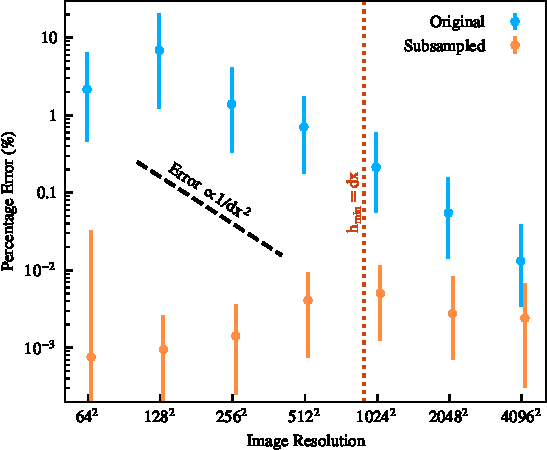
\includegraphics[width=\columnwidth]{./plots/gradient_2d/test_convergence.pdf}
  \caption{Compares the errors (in the 10\%, 50\%, 90\% percentiles from bottom, point, to top) for the original and subsampled method. Note that each point is evaluated at the number of pixels given on the horizontal axis, with them offset for clarity when the range bars overlap.}
  \label{fig:gradconv}
\end{figure}

In the final column the original approach has visually converged to the subsampled result, with each particle being spread over many pixels. In Fig. \ref{fig:gradconv} we show the numerical convergence, relative to a downsampled $8192^2$ grid.
This is used instead of the analytical solution to remove the impact of any shared systematics between the two approaches, such as the lack of limb brightening in our projected kernel. Percentage error $E_{\%}$ is calculated as
\begin{equation}
  E_{\%} = 100 \cdot \frac{|\rho_{\rm test} - \rho_{\rm ref}|}{\rho_{\rm ref}},
\end{equation}
with $\rho_{\rm test}$ the calculated density reconstruction in that pixel and $\rho_{\rm ref}$ the reference density. Each point shows the median absolute percentage error over all pixels, with the bar showing the 10-90 percentile range.

At all resolutions, the subsampled method ensures that the percentage error in the reconstruction is imperceptibly low, with a highest 90\% value of roughly 0.05\%. Notably, this does not decrease with resolution, as the method is designed to produce converged results at all grid sizes. The original method, on the other hand, demonstrates a high level of error with almost all pixels having at least a 1\% reconstruction error at $128^2$ resolution. This error does indeed converge at the expected rate ($1 / {\rm d}x^2$ as this corresponds to the number of pixels sampling each kernel), but even at the highest resolutions the subsampled approach still provides lower error due to its improved gradient reconstruction of particles with the smallest smoothing lengths (note that $10^{-3} \approx 5 / 4096$, so even at this high resolution the sub-pixel supersampling is still in effect for the highest densities).

\begin{figure}
  \centering
  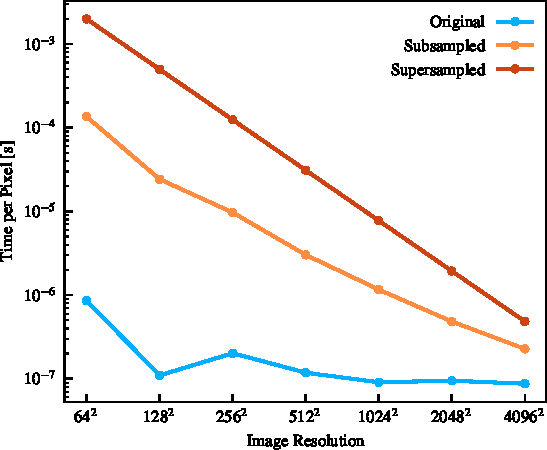
\includegraphics[width=\columnwidth]{./plots/gradient_2d/pixel_time_scaling.pdf}
  \caption{Time-to-solution (using four cores of an Intel i7-8559U) per pixel corresponding to the accuracy results in Fig. \ref{fig:gradconv} for three strategies: the original method with no subsampling (blue); the subsampled method (orange); and using a downsampled pixel grid originally calculated at 8192$^2$ (red). Here we see that although there is significant computational cost associated with the use of the subsampling strategy (along with, of course, the accuracy gains), it still remains approximately 10 times faster than downsampling a large grid.}
  \label{fig:gradtime}
\end{figure}

The improved reconstruction using the subsampling technique hence provides a significant increase in accuracy relative to traditional methods in an adaptive environment. This, however, comes at the cost of increased computing cycles. Fig. \ref{fig:gradtime} shows the scaling of the time to produce the projected density grid for points in Fig. \ref{fig:gradconv}. The red line shows, for comparison, the time taken to compute the $8192^2$ reference grid, which could be downsampled to provide a high accuracy reconstruction. The subsampled technique is still roughly an order of magnitude faster than this, thanks to its efficient handling of particles that are already spread over enough pixels to be well sampled.